\begin{explanationbox}
\begin{minipage}{\linewidth}
\begin{center}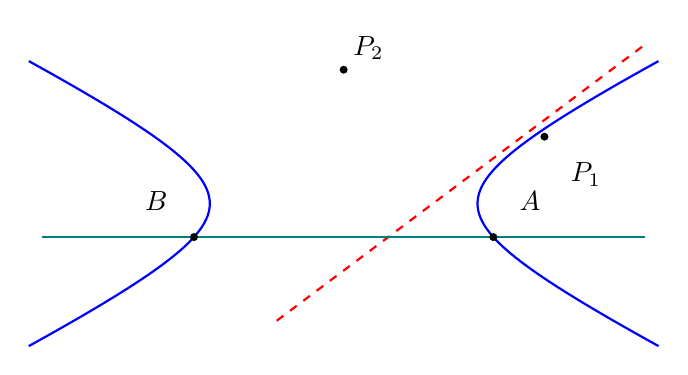
\begin{tikzpicture}[scale=0.85,>=stealth]
\draw[blue,thick,domain=-1.5:1.5,samples=90] plot ({2*cosh(\x)},{sinh(\x)});\draw[blue,thick,domain=-1.5:1.5,samples=90] plot ({-2*cosh(\x)},{sinh(\x)});\draw[red,dashed,thick] (-1,-1.75)--(4.5,2.375);\draw[teal,thick] (-4.5,-.5)--(4.5,-.5);\fill (3,1) circle (1.7pt) node[below right=6pt] {$P_1$};\fill (0,2) circle (1.7pt) node[above right] {$P_2$};\fill ({sqrt(5)},-0.5) circle (1.7pt) node[above right=6pt] {$A$};\fill ({-sqrt(5)},-0.5) circle (1.7pt) node[above left=6pt] {$B$};
\end{tikzpicture}
\end{center}
$P_1=(3,1)$ 的红色极线没有实交点；$P_2=(0,2)$ 的绿色极线 $y=-1/2$ 才是实际切点弦。二者不能只凭“外点”一词混同。
\end{minipage}
\par\medskip

	\textbf{\textcolor{CExplanation}{一句话直觉}}
	过双曲线外一点作两条切线，两个切点的连线（切点弦）的方程可以由该点的坐标直接代入一个固定形式得到，无需求出切点坐标。

	\medskip
	\textbf{\textcolor{CExplanation}{核心拆解}}
	\begin{description}[style=nextline, leftmargin=2.8em, labelsep=0.5em, itemsep=0.45em]
		\item[\textbf{要点一（代换规则）：}]
			切点弦方程与对应标准方程下的切线方程形式相同，只需将切线方程中的切点坐标替换为 $P(x_0,y_0)$ 即可。
		\item[\textbf{要点二（结构特征）：}]
			方程左侧为 $\frac{x_0 x}{a^2} - \frac{y_0 y}{b^2}$ 或 $\frac{y_0 y}{a^2} - \frac{x_0 x}{b^2}$，右侧恒为 $1$，与双曲线标准方程右端一致。
	\end{description}

	\medskip
	\textbf{\textcolor{CExplanation}{几何本质（两点连线）}}
	切点弦本质是两切点的连线，它通过 $P$ 点关于双曲线的极性关系确定。$P$ 是外部点，两切点的坐标满足双曲线方程，它们的连线恰好由该方程决定。

	\medskip
	\textbf{\textcolor{CExplanation}{代数意义（代换规则）}}
	将双曲线标准方程 $\frac{x^2}{a^2} - \frac{y^2}{b^2} = 1$ 中的 $x^2$ 替换为 $x_0 x$，$y^2$ 替换为 $y_0 y$，其余不变，即得到切点弦方程。这种“代一半”规则是二次曲线切线与切点弦的共性。

	\medskip
	\textbf{\textcolor{CExplanation}{考点价值（直接应用）}}
	\begin{itemize}[leftmargin=*, itemsep=0.5em, topsep=0.4em]
		\item \textbf{考法一（求切点弦方程）：} 给出双曲线方程和外部点坐标，直接套用公式写出切点弦方程。
		\item \textbf{考法二（逆向求点）：} 给出切点弦方程和双曲线方程，反解外部点 $P$ 的坐标。
	\end{itemize}

	\medskip
	\textbf{\textcolor{CExplanation}{顿悟点}}
	核心是记住代换模式：$x^2 \to x_0 x$，$y^2 \to y_0 y$，常数项 $1$ 不变。这种代换对椭圆和双曲线都适用，但双曲线的符号差异要注意（中间是减号）。

	\medskip
	\textbf{\textcolor{CExplanation}{使用场景}}
	\begin{itemize}[leftmargin=*, itemsep=0.5em, topsep=0.4em]
		\item \textbf{场景一（已知点求弦）：} 已知双曲线外一点 $P$，直接写出过 $P$ 的两切线的切点弦方程。
		\item \textbf{场景二（已知弦求点）：} 已知切点弦直线方程，通过比较系数求出 $P$ 点坐标。
	\end{itemize}

\textbf{两有限实切点的存在条件。}
记 $q=x_0^2/a^2-y_0^2/b^2$，则恰有两个不同的有限实切点当且仅当
$q<1$ 且 $q\ne0$。$q=1$ 是一个切点，$q>1$ 无实切点；
$q=0$ 的非中心点在渐近线上，只有一个有限切点，另一方向为渐近线；中心点没有实切线。
纵轴形式使用 $q=y_0^2/a^2-x_0^2/b^2$。
\end{explanationbox}
